To fulfil the requirement specification\ref{sec:reqspec} of making a working prototype a GUI (Graphical User Interface) have been created. 

\textbf{Making a sketch:}\\
The basic idea behind the GUI was drawn up as a sketch which can be seen in \ref{fig:guisketch} . The creation of very lo-fi prototype was only to understand what to implement and have a discussion about functionality.

\begin{figure}[H]
\begin{center}
\leavevmode
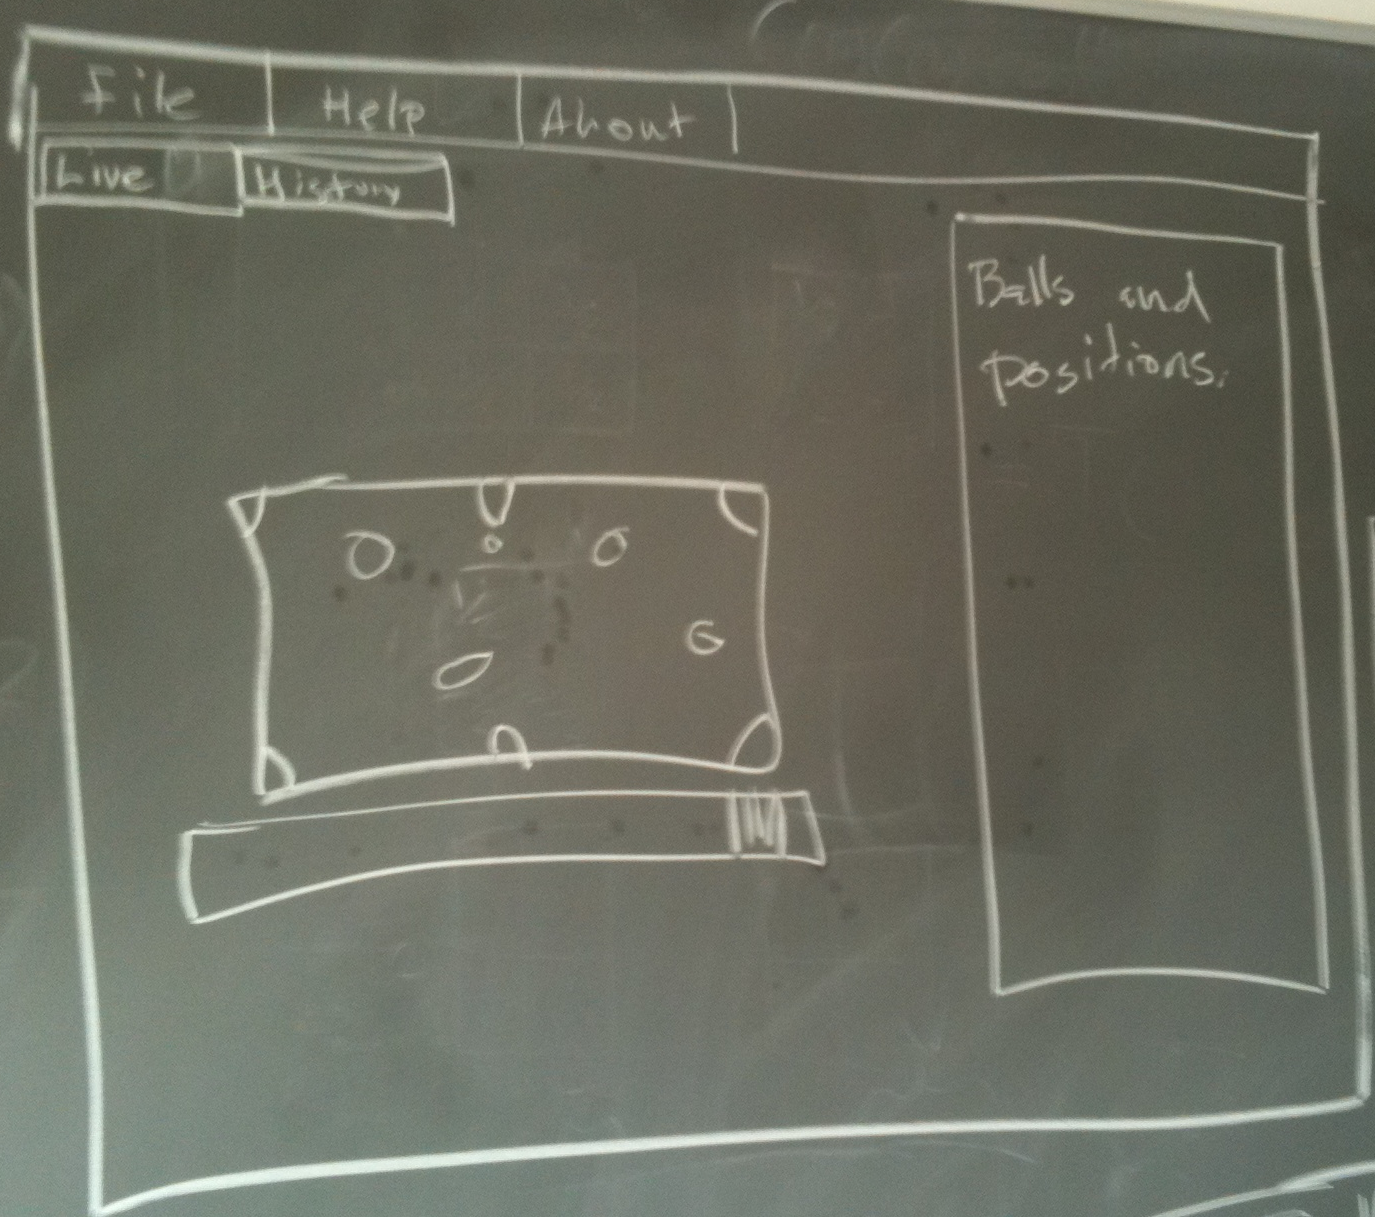
\includegraphics[width=0.5\textwidth]{images/guisketch}
\end{center}
\caption{A sketch of GUI on a blackboard.}
\label{fig:guisketch}
\end{figure} 

\textbf{Implementation:}\\
The implementation was done in Visual Studios C\# 2010 using the sketches. 

\fixme{indsæt tegninger}

\textbf{Using the prototype:}\\
The prototype is build using the PoolTracker library created in this project. The GUI created in one solution and the library is integrated as another solution. This allowed for the development to be done simultaneously and for easy integration into other projects.\\
The prototype consists of the following files:
\begin{itemize}
	\item pooltracker.exe : The executable prototype.
	\item config.xml	  : The config-file which contains calibration settings.
	\item pooltracker.dll : The PoolTracker library.
	\item EMGU FIIILES!!  : Aaaaal the files used!
\end{itemize}

Simply connect a webcam and place it above your pool table. Then run the prototype, calibrate and start playing.